\chapter{\MakeUppercase{Обзор литературы}}
\label{ch:chap1}

В первой главе рассматривается...

\section{По ФРК и кровотоку}
Стеноз коронарных артерий -- это патологическое сужение просвета сосудов, ответственных за кровоснабжение сердца (Рисунок {\ref*{fig:1}}). При значительно уменьшении диаметра артерии развивается ишемия миокарда, которая проявляется стенокардией, одышкой, а в критических случаях -- инфарктом. Основной причиной возникновения стенозов является атеросклероз - хроническое заболевание, при котором на внутренних стенках сосудов формируются холестериновые бляшки. Эти образования состоят из липидов, кальция и соединительной ткани. Со временем бляшки увеличиваются, нарушая кровоток, а их разрыв может спровоцировать риск тромбоза и полной закупорки сердца.

  
Стентирование -- инвазивная операция, направленная на восстановление проходимости крови в пораженной артерии. Выполняется под местной анестезией через прокол в бедренной или лучевой артерии, через который под рентген-контролем вводится катетер к сердцу. После ангиографии с контрастным веществом, выявляющей локализацию и степень стеноза, выполняется баллонная ангиопластика: миниатюрный баллон раздувается в зоне сужения, восстанавливая просвет сосуда. Затем имплантируется стент — металлический сетчатый каркас, предотвращающий рестеноз. Современные стенты с лекарственным покрытием снижают риск разрастания рубцовой ткани.


Для определения функциональной значимости стеноза перед вмешательством используется фракционный резерв кровотока (ФРК) -- гемодинамический индекс, оценивающий градиент давления до и после сужения. 

\begin{equation}\label{eq:e1}
	FFR = \frac{P_d}{P_a},
\end{equation}
где $P_d$ -- давление крови после стеноза, $P_a$ -- давление в аорте.

\begin{figure}
	\centering
	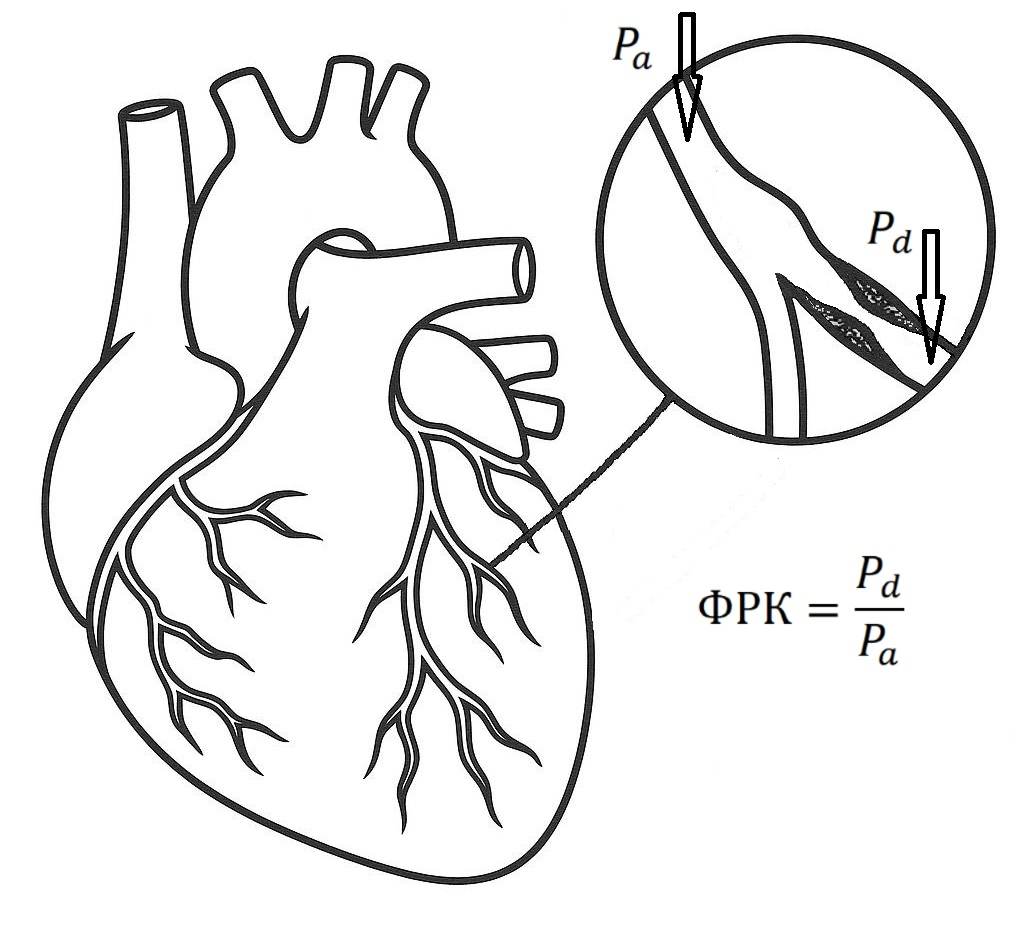
\includegraphics[]{images/chap1/FFR_dem.jpg}
	\caption{Стеноз левой коронарной артерии.}
	\label{fig:1}
\end{figure}
%\hyperref[fig:dicom]{рисунке \ref*{fig:dicom}}

ФРК помогает выявить, вызывает ли стеноз ишемию миокарда: значение ≤ 0.8 указывает на необходимость стентирования, что повышает точность отбора пациентов и снижает риск избыточных вмешательств. Для определения ФРК в медицинской практике используют инвазивные методы с использованием провокационных тестов. Введение вазодилататоров (сосудо-расширяющих препаратов), таких как аденозин или папаверин, вызывает гиперемию -- усиление кровотока, что позволяет измерить давление до и после сужения артерии с помошью специального датчика (Рисунок {\ref*{fig:2}}). Этот тонкий проводник с датчиком давления продвигается через катетер к пораженному участку артерии, регистрируя изменения в реальном времени. Ангиограмма, совмещенная с данными ФРК, визуализирует зону ишемии, обеспечивая точное планирование операции.

\begin{figure}
	\centering
	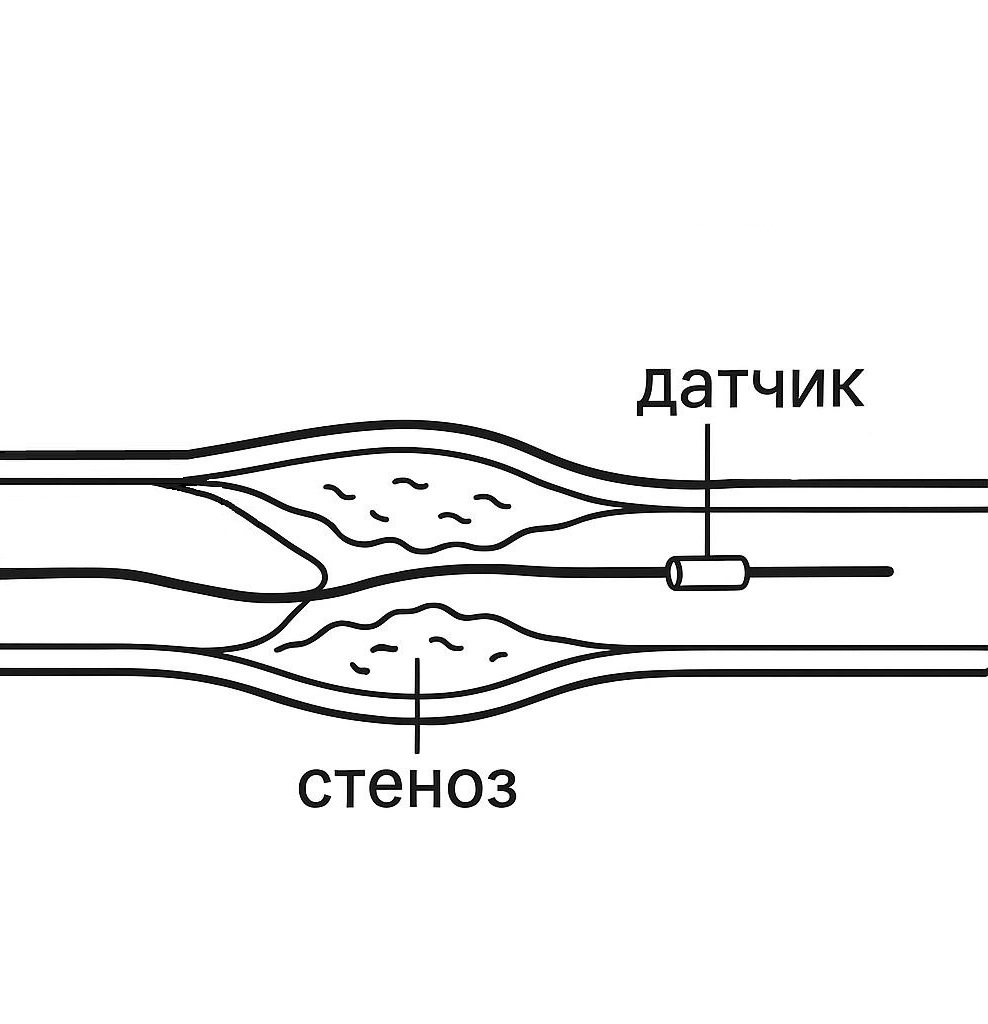
\includegraphics[]{images/chap1/pressure_wire.jpg}
	\caption{Введение катетера с датчиком давления в область стенозированного участка артерии.}
	\label{fig:2}
\end{figure}

Существует и альтернативный способ измерения ФРК -- с помощью математических моделей кровотока. Данный метод не требует инвазивного хирургического вмешательства и позволяет с некоторой погрешностью оценивать значение давления в артериях. Часто используются модели [Ссылки на модели], использующие данные компьютерной томографии (КТ), на основе которых строится 0D/3D модель коронарных артерий в которой с помощью алгоритмов гидродинамики прогнозируются характеристики тока крови.Точность таких расчетов достигает X [Ссылка на статью с точностью], что сопоставимо с инвазивным методом, но без рисков катетеризации.

Клиническая значимость ФРК:
{Согласно рекомендациям ESC/ACC, FFR <0.8 является ключевым критерием для принятия решения о реваскуляризации. Исследование FAME доказало, что FFR-ориентированная стратегия снижает риск основных сердечно-сосудистых событий (MACE) на 30\% по сравнению с ангиографическим подходом. Алгоритм включает этапы: оценка симптомов → ангиография → измерение FFR → стентирование при FFR ≤0.8.}


Ограничения ФРК:
{Несмотря на высокую точность, FFR имеет ограничения. Микрососудистая дисфункция (например, при диабете или гипертонии) может искажать результаты: в таких случаях FFR остается нормальным, но стресс-тесты выявляют ишемию из-за нарушения вазодилатации мелких сосудов. Это явление называют «диссоциацией FFR и ишемии», что требует комплексной оценки с использованием дополнительных методов (например, индекса микрососудистого сопротивления).}

Картинка : Схема микрососудистой дисфункции (сравнение здоровых и пораженных микрососудов).

\iffalse
\begin{figure}
	\centering
	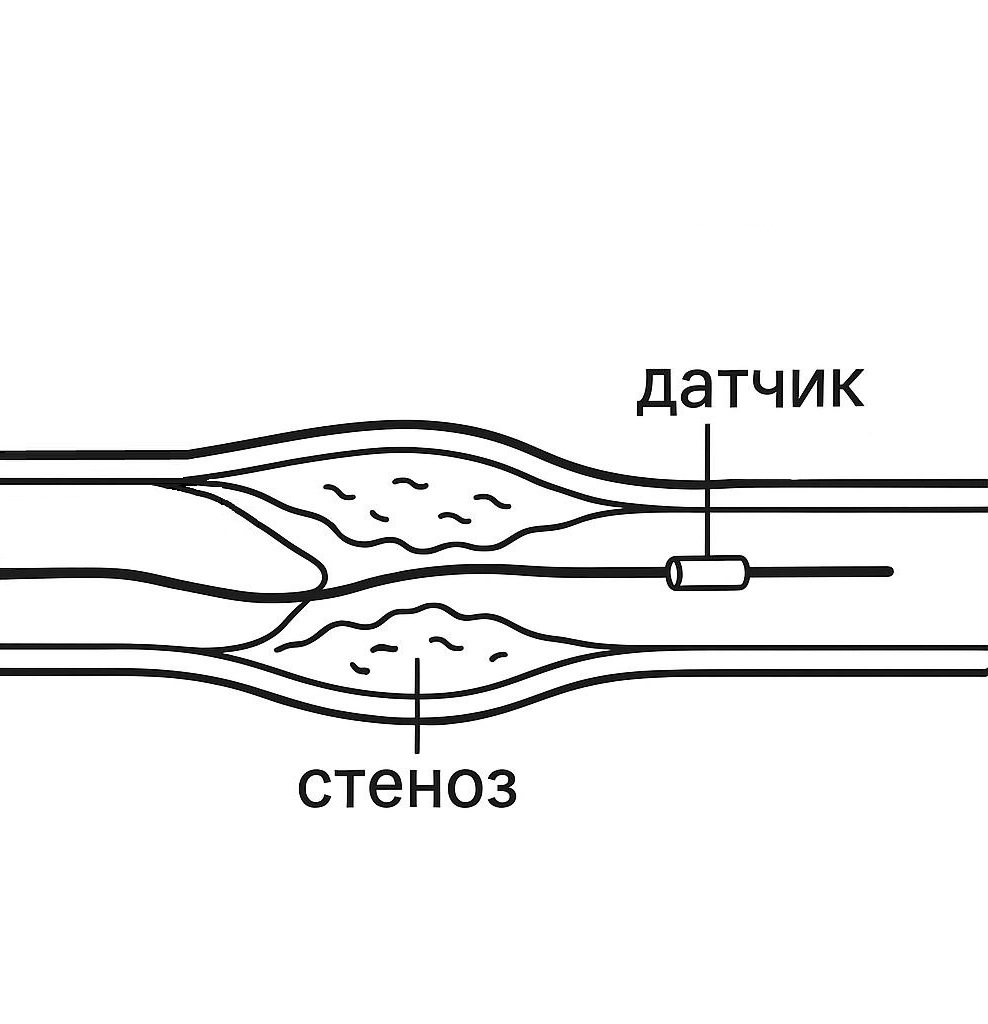
\includegraphics[]{images/chap1/pressure_wire.jpg}
	\caption{Сравнение здоровых и пораженных сосудов.}
	\label{fig:2}
\end{figure}
\fi

\section{По моделям для вычисления ФРК}
Современные модели кровотока позволяют...

% \subsection{Подсекция, в которой мы демонстрируем, как выглядят многоуровневые нумерованные списки}

%     Теперь попробуем разобраться с нумерованным списком. Его можно делать многоуровневым, при этом нам важно соблюдать формирование по ГОСТ: в подпунктах используются буквы русского алфавита (все, кроме ё, з, й, о, ч, ь, ы, ъ). Необходимое форматирование уже задано в основном файле. Выглядеть это будет так:

%     \begin{enumerate}
%         \item Первый пункт
%         \begin{enumerate}
%             \item Первый подпункт первого пункта
%             \item Второй подпункт первого пункта
%         \end{enumerate}
%         \item Второй пункт
%         \begin{enumerate}
%             \item Первый подпункт второго пункта
%             \item Второй подпункт второго пункта
%             \begin{enumerate}
%                 \item Это уже подпункт третьего уровня
%                 \item Сделаем еще один подпункт третьего уровня. Он будет достаточно большим, чтобы показать, как текст в нумерованном списке переносится на следующую строку
%             \end{enumerate}
%             \item Третий подпункт
%         \end{enumerate}
%     \end{enumerate}

% \section{Метки и ссылки}

% В \LaTeX{}е достаточно большие возможности для создания различного рода ссылок в тексте. Можно ссылаться на любые места, страницы, рисунки, таблицы, разделы и т.д., и \LaTeX{} сам подтянет нужный номер и/или имя. Для задания красивых ссылок мы пользуемся пакетом \verb|hyperref|. Важно помнить, что для этого обязательно надо поставить метку. Ссылка на \nameref{ch:intro}, например, не будет работать, если после объявления данной главы в коде не поставить на него метку. 

% Кроме того, можно поставить метку в любом месте, к которой потом можно обратиться с помощью специальных команд \verb|ref| и \verb|hyperref|. Первая возвращает \textbf{только кликабельный номер} раздела, рисунка, формулы, т.д. (если он доступен), а вторая позволяет делать гиперссылкой любое слово или текст, а также совмещать текст с автоматически подгружаемым номером. Например,  при помощи \verb|hyperref| мы можем сделать красивую ссылку на \hyperref[sec:fig]{Раздел \ref{sec:fig}}, в котором мы разберем, как делать рисунки и подрисуночный текст. Можно было бы воспользоваться просто командой \verb|ref|, тогда ссылкой был бы только номер, без слова "<Раздел">: Раздел \ref{sec:fig}.

% \section{Библиография}

% С библиографией в \LaTeX{}е все просто: вставляете ссылки из Google Scholar в формате bibtex в \verb|.bib|-файл, назначаете им \verb|citekey| (это по сути те же уникальные метки, только для ссылок в списке литературы) и отмечаете их в тексте, где надо процитировать одну или несколько работ. Если копировать из Google Scholar, то \verb|citekey| назначаются автоматически. Цитирование и оформление библиографии делается при помощи пакета \verb|biblatex|, а формат ссылок задается в основном файле. Для примера в шаблоне уже есть \verb|.bib|-файл с несколькими ссылками. Попробуем их процитировать и посмотреть, как это будет выглядеть в документе. Например, сделаем ссылку на учебное пособие по наноструктурам \cite{федоров2014физика}. А теперь сделаем двойную ссылку на него и на еще одну работу \cite{ozaki2019ozaki}. Можем сразу несколько процитировать \cite{gaponenko1998optical,федоров2014специальные,гапоненко2005оптика,калитеевская2018выделение}. Наконец, процитируем пару иностранных статей, чтобы посмотреть как будут выглядеть англоязычные работы \cite{dhamo2021efficient} в нашей библиографии \cite{miropoltsev2022influence,dey2021state}. Согласно ГОСТ, формат ссылок (то есть, записи типа "<и др.">, "<Том">) должны соответствовать языку цитируемой работы. То есть, если цитируете статью или книгу на английском --- то в записи должно быть "<et al.">, "<Vol."> и так далее. В данном шаблоне реализовано автоматическое определение языка ссылки по наличию в названии работы символов кириллицы. При этом, если \LaTeX{} что-то перепутал, вы всегда можете задать значение полей \verb|langid| для записей в \verb|.bib|-файле вручную, тогда программа выберет именно тот язык, который вы указали. \textbf{Важно!} Для других языков типа немецкого, испанского и т.д. надо подгружать дополнительный функционал через пакет \verb|babel|. С другой стороны, обычно в таких случаях достаточно использовать английский.

\endinput